\documentclass[11pt]{article}
\usepackage{amsmath, amsfonts, amsthm, amssymb}  % Some math symbols
\usepackage{enumerate}
\usepackage{fullpage}
\usepackage[x11names, rgb]{xcolor}
\usepackage{tikz}
\usepackage{graphicx}
\usetikzlibrary{snakes,arrows,shapes}
\usepackage{wasysym}
\usepackage{dsfont}
\usepackage{centernot}

\setlength{\parindent}{0pt}
\setlength{\parskip}{5pt plus 1pt}
\pagestyle{empty}

\def\indented#1{\list{}{}\item[]}
\let\indented=\endlist

\newcounter{questionCounter}
\newcounter{partCounter}[questionCounter]

\newenvironment{question}[2][\arabic{questionCounter}]{%
    \addtocounter{questionCounter}{1}%
    \setcounter{partCounter}{0}%
    \vspace{.25in} \hrule \vspace{0.5em}%
        \noindent{\bf #2}%
    \vspace{0.8em} \hrule \vspace{.10in}%
}{}

\renewenvironment{part}[1][\alph{partCounter}]{%
    \addtocounter{partCounter}{1}%
    \vspace{.10in}%
    \begin{indented}%
       {\bf (#1)} %
}{\end{indented}}

%%%%%%%%%%%%%%%%% Identifying Information %%%%%%%%%%%%%%%%%
%% This is here, so that you can make your homework look %%
%% pretty when you compile it.                           %%
%%     DO NOT PUT YOUR NAME ANYWHERE ELSE!!!!            %%
%%%%%%%%%%%%%%%%%%%%%%%%%%%%%%%%%%%%%%%%%%%%%%%%%%%%%%%%%%%
\newcommand{\myname}{Michael Rosenberg}
\newcommand{\myandrew}{mmrosenb@andrew.cmu.edu}
\newcommand{\mycourse}{73-449: Social, Economic, and Information Networks}
\newcommand{\myhwname}{| Final Project Report}
\newcommand{\myrecitation}{Anderson, Section A}
\newcommand{\myteammates}{}
\newcommand{\Z}{\mathds{Z}}
\newcommand{\bigdot}{\textbf{.} }
\newcommand{\spa}{\hspace{2cm}}
\newcommand{\proposition}{\textbf{\underline{Proposition:} }}
\newcommand{\proofwrite}{\textbf{\underline{Proof.} }}
\newcommand{\claim}{\textbf{\underline{Claim.} }}
\newcommand{\AFSOC}{Assume for the sake of contradiction }
\newcommand{\theorem}{\textbf{\underline{Theorem:}} }
\newcommand{\definition}{\textbf{\underline{Definition:}} }
\newcommand{\xNot}{\mathbf{x}_0}
%%%%%%%%%%%%%%%%%%%%%%%%%%%%%%%%%%%%%%%%%%%%%%%%%%%%%%%%%%%%%%%%%%%%%%%%%%%%%%%%

\begin{document}
\begin{center}
    {\Large \mycourse} {\Large \myhwname} \\
    \myrecitation \\
    \myname \\
    \myandrew \\
    %\myteammates 
\end{center}

A tax haven is a jurisdiction where a given individual or company can get a
more favorable tax rate on the exchange of goods and capital than another
jurisdiction. Typically, a tax haven is represented as a country with a
favorable tax regime, although it can often be a territory embeded within a
country. Individuals and companies often want to set up entities within tax
havens for two reasons. The first reason is that the favorable tax regime within
a tax haven is often helpful for retaining a large amount of financial assets
within a company. The second reason is that tax havens typically have looser
laws on financial transparency when compared to other jurisdiction, and so
companies and individuals can use entities and tax havens to perform
transactions in a less regulated environment than their typical jurisdiction.

Tax havens have been a source of controversy in developed and middle-income
countries in recent years. Governments have been worried by the many large
private institutions that choose to set up entities within tax havens such as
Switzerland, the Bahamas, and Panama. This worry comes from two reasons. The
first reason is that when companies set up entities within these tax havens, a
lot of tax revenue that would come from domestic financial transactions is lost
due to the offshoring of certain parts of the business; this is often looked at
by government as a form of tax evasion. The other reason is that the lack of
financial transparency in these tax havens allows certain informal economies to
develop around the world, such as the financial backing of the drug trade.

When I first looked at this problem, I saw that the relationships formed by
domestic companies and individuals and offshore entities to be graphical in
nature, and so I found that the questions facing the use of tax havens to be
network analysis questions. My first question is, what aspects of the tax haven
network give legal and financial intermediaries social capital in the network?
If we are able to identify these aspects of the network, we would be able to
identify the responsibility that domestic intermediaries have in holding up the
connections of offshore entities. My second question is, what are some policy
interventions we can do to reduce the strength of this network? If we begin to
build some of these policy interventions, we may be able to find mechanisms to
reduce global tax evasion and fight illicit economies.

The source of my data comes from International Consortium of Investigative
Journalists (ICIJ). ICIJ is a non-governmental organization that was developed
by the Center for Public Integrity as a group that would connect investigative
journalists from around the world. This organization has created the Offshore
Leaks Database, a graph database that displays the major players in the
financing and operation of tax haven entities and the relationships among these
players. This database was formed by ICIJ over three document leaks. The first
leak was the Offshore (China) Leaks, a document leak in 2013
that detailed tens of thousands of tax haven clients from Hong Kong and 
Mainland China. The second leak was the Panama Papers, a leak in May of 2016
that featured the financial dealings of major players across the developed
world's richest individuals. The last leak was the Bahamas Leaks, a cache of
documents that was exposed in September of 2016 that contained the financial
transactions of hundreds of thousands of Bahamian entities.

This dataset
\begin{figure}[h!]
    \centering
    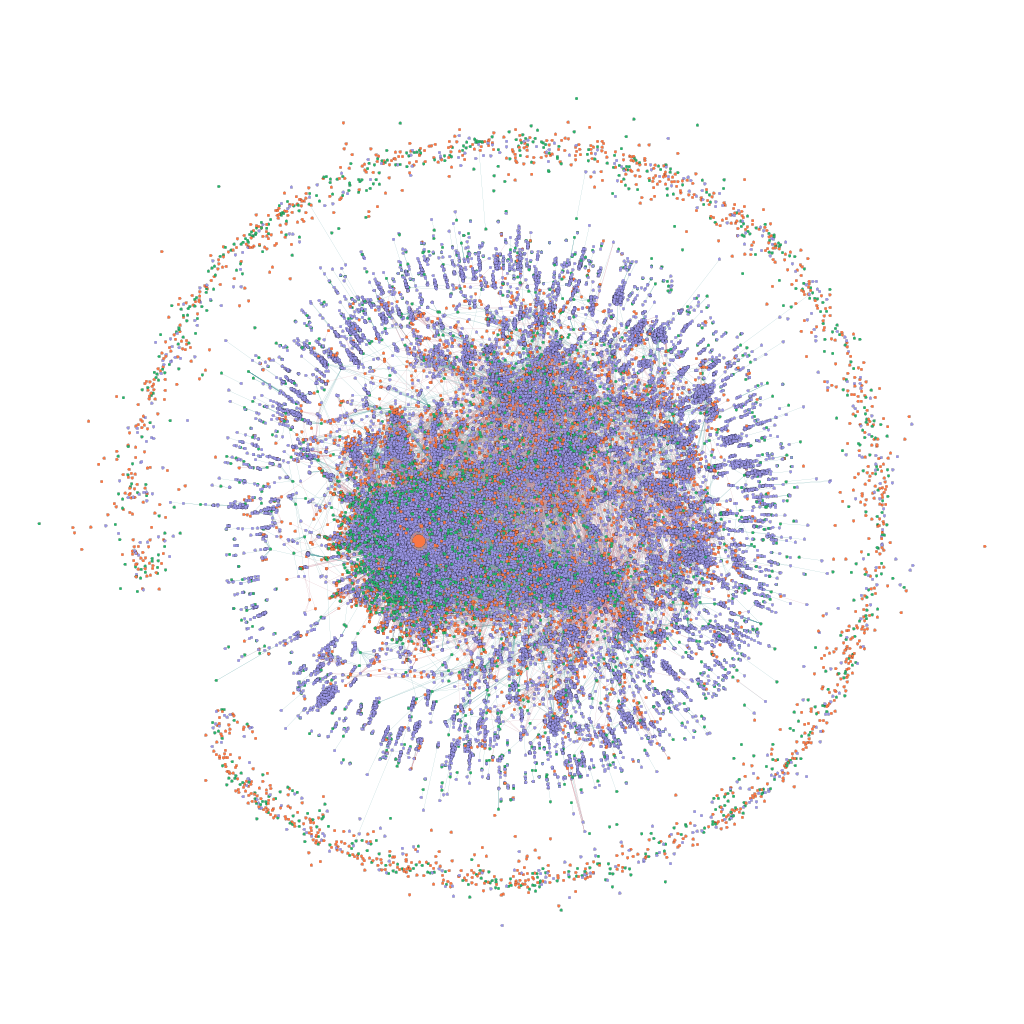
\includegraphics[width = 5in]{figures/figure1.png}
    \caption{A visualization of our final dataset with the removal of
            nodes with a degree of less than $5.$ Nodes are sized by
            degree and nodes are colored by agent type, where entities are
            purple, officers are orange, and intermediaries are green.}
\end{figure}

\end{document}
